\addcontentsline{toc}{chapter}{Software}
\chapter*{Software}

 %%%%%%% INTRODUCTION %%%%%%
%\addcontentsline{toc}{section}{Introduction}
%\section*{Introduction}
In this section the software developed in this Bachelor's Thesis is presented and thoroughly explained. 
\\

The code was created as a ROS package. ROS (Robotic Operating System) is an Operating System designed to be implemented in robots. It has libraries to enhance the communication between nodes, the processes management or the threads present in the code among other functionalities. 
Since this code is intended to be running on a robot, the software developed was created as a ROS package. 
\\

In order to manage 2D and 3D information (images and pointclouds) two libraries has been used: OpenCV and PCL. Those two libraries implement basic and state-of-the-art algorithms that allow a easier and more time-efficient management of the data. 
\\

The software was structured in nodes. These nodes have a relatively small functionality and run in parallel. The fact that they run simultaneously improves the efficiency of the code lowering the lag due to time-expensive operations. 
\\

In the following sections, the software structure and tools used are described. 


\newpage

 %%%%%%% SOFTWARE STRUCTURE %%%%%%
\addcontentsline{toc}{section}{Software structure}
\section*{Software structure}

%In this section, the code functionalities of each part or node of the software are explained. The communication between nodes is shown and the overall software flow is thoroughly described. 

The code is structured in nodes. Each node contains a piece of the processing needed in the code. All nodes are related between them using ROS messages to transport the input and output data. 
\\

Computer vision is a field that involves high time-expensive algorithms. In the previous chapter it was explained that it uses 2D and 3D information. That information implies a matrix that has for each point 2 coordinates number (in the case of 2D) or 3 coordinates (in the case of 3D data), apart from the colour of that point, which is described using 3 more integers. \\

As it can be seen the data handled is enormous an the way to reduce the time lag due to those computations is modularizing the computation and executing in parallel those processes. 
\\

The software was designed to be as modular as was possible so that each node performs an action that could be used in other applications. 
As an example, the code could be easily changed to recognize hats or shoes, just changing the initial node that extracts the information of the desired joint. 
\\

In the following paragraphs the nodes' functionalities will be described and the communication between them presented. But first, the overall software work-flow is shown using the flow diagram below. 

\newpage
 %%%%%%% SOFTWARE FLOWCHART %%%%%%
\addcontentsline{toc}{subsection}{Software flowchart}
\subsection*{Software flowchart}

The input of the system is the information coming from the RGB-D sensor. There are two different data that are taken: the 2D information, i.e. the raw image detected by the sensor's camera, and the 3D information, i.e. the raw point cloud. Also, there is another input to the system that shows the position of the different user's joints. This data is provided by a third-party package called pi\_tracker that is explained in the following chapters. 
\\

The software was designed to be running on a robot as was previously explained. This implies that there can not be a GUI (G** User Interface) on a screen because the robot being used might not have it. Also, the usability and easiness to learn how to interact with the program was important to allow different people not only investigators to use it. 
\\

In order to fulfil those requirements a gestural interface was designed. It is developed by a separate node so the processing lags will not affect the recognition of the different gestures. This fact also allows an easy change of the gestures being used. 
\\

The recognition of the location of the hand with respect to the user's body shows how the arm is positioned. If it is stretched towards the sensor, the software enters the dataset construction mode, i.e. the data acquisition and learning mode. If, otherwise, it is located closer to the body, the software starts the object recognition mode. 
\\

\begin{figure}[h]
	\begin{center}
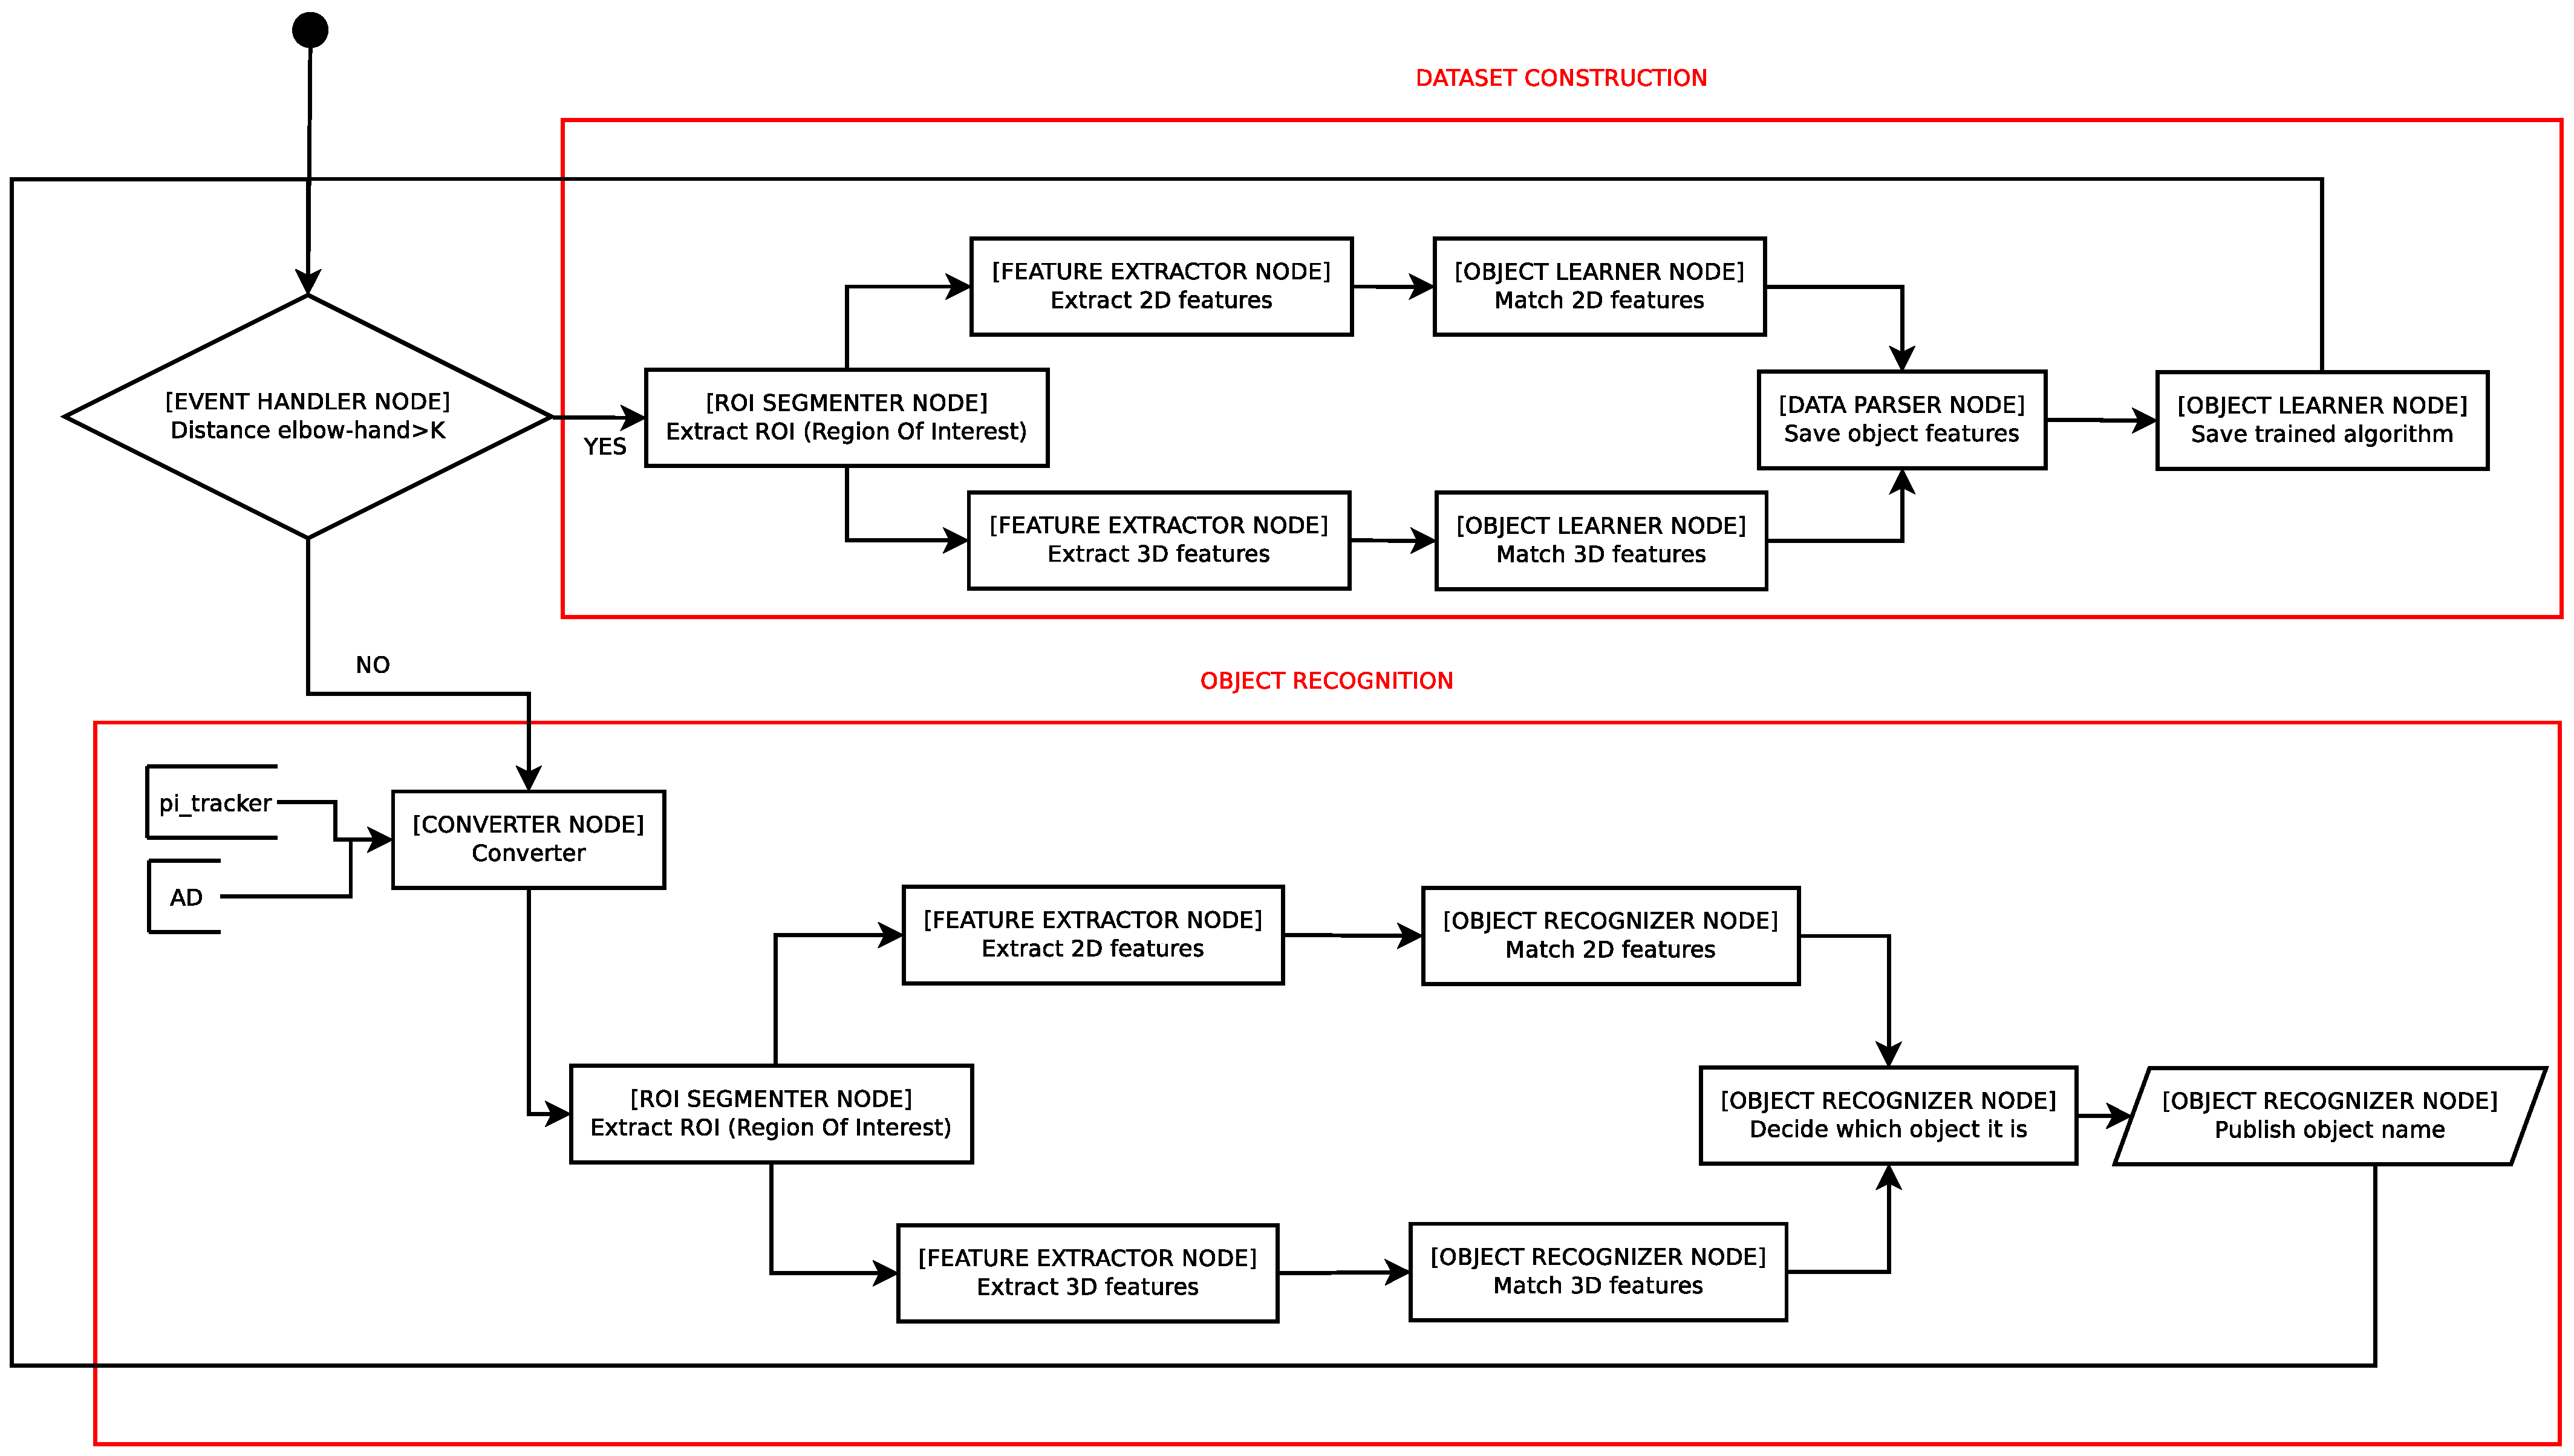
\includegraphics[scale=0.2]{img/diagrams/flowcharts.eps}
	\caption[Software flowchart]{Complete Software flowchart showing the different processing steps between the input and the output}
	\end{center}
\end{figure}


The upper part of the diagram shows the data acquisition work-flow. The first step is to extract the ROI (Region of Interest) from the input raw data. This is a crucial step that allows to reduce noticeably the amount of time due to computation reducing the size of the processed information. 
\\

After the extraction, the 2D and 3D features of the segmented data are obtained. The features or descriptors are characteristics that define and represent the data from where they were created. There are different algorithms that perform this task with better or worse repeatability and robustness. All the details about this process is explained in the next chapters. 
\\

That is the end of the data cycle of the learning process. It is iterated over the number of views for each object that is required in order to obtain all the templates necessary per object. 
\\

The recognition mode was triggered when the hand was located near the user's body. This mode can be seen in the lower part of the previous diagram. 
\\

The steps that compose this part of the software are the following: 
First, the input information is converted to the custom message used within the code. Afterwards, as in the previous mode, the Region Of Interest is segmented from both 2D and 3D original information. Then, the descriptors are extracted exactly the same way as in the previous mode. 
\\

The next step is the recognition algorithm. This matches the descriptors from both the image and the point cloud and decides which object of the dataset is more similar to the one that is currently on the user's hand. More details about this algorithm may be found in this section. 
\\

Finally, the object identification number is obtained. This data is the output of the system. 

\newpage
%%%%%%% TOOLS %%%%%%
\section{Libraries and technologies}
\label{libraries_and_technologies}

This section covers the different libraries and technologies used in the development of this thesis. First, the programming framework present in the project's progression is displayed, as well as the different third-party libraries and packages that has been employed in the software. Afterwards, the tools used for profiling and testing the code are analyzed and, finally, the hardware being used is presented and its main characteristics explained. 




	\subsection{ROS}
		\label{ros}

	ROS is the acronym of Robot Operating System\cite{ros}. It is an open source set of libraries and various tools that are aimed at robot applications. It is intended as well to improve the efficacy of collaborative robotics development, allowing easy interconnection of ROS packages. 


	\begin{figure}[h]
		\begin{center}
	    
\includegraphics[scale=0.3]{img/ros/groovy.eps}
		\caption[ROS Groovy Logo]{ROS Groovy Logo}
		\end{center}
	\end{figure}

	The tools, libraries and third-party packages available in the different ROS distributions are very useful when programming software for a robot. This is the main reason why this Operating System was selected as the framework in which develop the code of this Bachelor's Thesis. 
	\\
	The structure of the software is detailed in the chapter \ref{system_design}.  It is a node structure in which different processes are executed in parallel in order to improve the efficiency of the code. Each node executes a different computation in the data-flow. 
	\\
	Since each node is part of a chain of information between the input and output of the system, they must be connected. This information sharing is produced using the ROS topics. 
	The ROS nodes are simply executables that uses the ROS messaging system to communicate with other nodes. The ROS topics are a messaging units in which the nodes can publish messages. Also, the nodes may subscribe to those topics in order to retrieve the messages already published on them. 
	\\
	The messages are pieces of data that the nodes send to each other. In ROS, the messages might be customized combining the already defined standard messages and sensor messages to create the message with the information needed. 
	%In this project various custom messages has been defined. More information about those can be found in the \ref{software_messages} section. 


		% \paragraph{ROS package: openni\_camera / freenect\_camera}\mbox{} \\

		% These two ROS packages are the RGB-D sensors drivers. Both can be used just changing the name of the executable or launch file. This is due to the fact that both publish the same information in identic topics. 
		% \\

		% They are needed in order to connect the kinect to the computer. They transfom the raw output information of the computer into a ros message with the different images and point clouds. 
		% \\

		% In this project both have been used indistinctly.  

		% \paragraph{ROS package: openni\_launch / freenect\_launch}\mbox{} \\

		% These packages take as the input the information provided by the openni\_camera / freenect\_camera. They provide useful transformations and a launch file that executes nodelets with that information. This way, not only the raw image and point cloud from the kinect can be obtained but also the registered point cloud or the disparity image. 
		% \\

		% Both have been used in the code and they are the input to the pi\_tracker package which is explained in the next section. They are the input of the system as well, providing the point clouds and images that are later on segmented by this software. 


		% \paragraph{ROS package: pi\_tracker}\mbox{} \\

		% This package was developed by an MIT group. It publishes in the output a relation of the position and pose of each joint of the user. It is capable of recognizing more than one person at a time and to give the information about it. 
		% \\

		% The package easies the hand tracking algorithm since the input to it is the hand's position. It is very helpful to determine gestures made by the user due to the completeness of the information provided. 
		% \\

		% In order to publish the information about the joints, a custom message pi\_tracker/Skeleton is created. 

	\subsection{Open Source Computer Vision (OpenCV)}
	\label{opencv}

	%Intro
	OpenCV\cite{opencv} is a library that implements state of the art real-time computer vision 
	algorithms. 

	It is cross-platform and it is released under a BSD\cite{BSD} license. 
	Figure \ref{opencv_logo} shows the logo of the OpenCV library. 
	% Previously it was integrated in ROS \cite{ros}, but now it is used as a stand-alone library.  

	\begin{figure}[h]
		\begin{center}
	    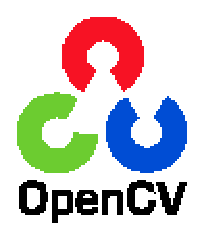
\includegraphics[scale=1]{img/opencv/logo.eps}
		\caption[OpenCV Logo]{OpenCV Logo}
		\label{opencv_logo}
		\end{center}
	\end{figure}

	The qualities described above as well as its optimization of various algorithms make this library an extremely useful asset for robotic vision projects. 
	In this project the C++ interface of the OpenCV library has been used. 
	The functionalities provided by this library are used in all the 2D data processing. 
	The next paragraph details the operations for which this library has been used. 

		\begin{itemize}
		\item\textbf{Segmentation of the 2D ROI (Region Of Interest)\\ }

		This library allows to crop the original raw image coming from the RGB-D sensor. 
		In our application, the segmentation is done around the user's hand. 
		For further details please read section \ref{roi_segmenter_2d}. 
		

		\item\textbf{ {Keypoints and descriptors extraction\\ }}

		 The OpenCV library implements multiple optimized state of the art algorithms. 
		 Among them, there are a number of descriptor extractors that has been already presented in chapter \ref{state_of_the_art}. 
		 The Oriented FAST and Rotated BRIEF (ORB)\cite{orb} algorithm is being used in this project due to its open-sourceness, and robustness / speed relation. 
		 More information about the different algorithms implemented in OpenCV used to extract the descriptors can be found in section \ref{feature_extraction}.


		\item\textbf{ {Descriptors matching\\ } }

		There are different matchers that might be used and that are implemented in the OpenCV library.
		The FlannBasedMatcher and the BruteForceMatcher are the two most used matchers due to its speed. 
		In this project, a FlannBasedMatcher (Fast Library for Approximate Nearest Neighbors Based Matcher) is being used for this purpose. 
		It is faster than the BruteForceMatcher specially for larger datasets. 
		It was selected to allow the use of more objects without losing efficiency. 
		\end{itemize}

	\subsection{Point Cloud Library (PCL)}
\label{pcl}
PCL is a standalone library that is open source and implements state-of-the-art algorithms related to 2D and 3D image and point cloud processing. \\
\begin{figure}[h]
	\begin{center}
    \includegraphics[scale=0.1]{img/pcl/pcl_logo.png}
	\caption[PCL Logo]{PCL Logo}
	\end{center}
\end{figure}

It is released under a BSD license, being free for commercial and research use. Is cross-platform and currently has been successfully compiled on Linux, MacOS, Windows, Android and iOS. \\

The library is divided in smaller code libraries that can be compiled separately. This modularity allows the PCL introduction on platforms with size constrains or that has a reduce computational size. \cite{Rusu_ICRA2011_PCL}
\\



\begin{figure}[h]
	\begin{center}
    \includegraphics[scale=0.4]{img/pcl/pcl_dependency.png}
	\caption[PCL graph of libraries]{PCL graph of code libraries and their relations}
	\end{center}
\end{figure}

		The Point Cloud Library is used within the software to perform transformations in the input point clouds and to perform descriptor extraction and matching in this data. 
		\\

		More specifically, PCL is used in the following processes: 

		\begin{itemize}
			\item{\textbf{Segmentation of the ROI (Region Of Interest)\\ }}

			This library allows to crop the original raw point cloud coming from the RGB-D sensor. In this application, the region cropped is the one around the hand being used. More information about this operation can be found in the \ref{roi_segmenter_3d} section. 
			

			\item{\textbf{ Keypoints and descriptors extraction\\ }}

			 The PCL library implements multiple optimized state of the art algorithms. Among them, there are a number of descriptor extractors such as PFH, FPFH or LINEMOD. In this project, the PFH descriptor is used due to its speed. More information about the different 3D descriptors implemented in PCL can be found in the section  \ref{feature_extraction}.


			\item {\textbf{Descriptors matching\\ }}

			There are different algorithms that allow to match the information provided by the descriptors, such as knn search or radius search. For further information about the type of matcher used in the present thesis, please visit the section \ref{learner_recognizer}
		\end{itemize}



	\subsection{Hardware}
		\label{technologies_hardware}

		The hardware needed in order to retrieve three-dimensional information is an RGB-D sensor compatible with the openni\_launch ROS package previously mentioned, and a computer running Linux. The information provided by this kind of device is more complete and makes the segmentation of the Region Of Interest easier. \\

		The sensor being used for the experiments presented in the following chapter is a Kinect of the Xbox 360. The reason of choosing this specific sensor is that it is cheaper than the other devices that include depth information. The main drawback with respect to other sensors such as the Asus Xtion PRO LIVE\cite{xtion} is that it needs a separate power plug to work, and also its size is bigger. 
		\\


		%  In this section the main components and functioning principles of the Kinect are going to be presented. Most of them are common with the other RGB-D sensors but others such as the VGA camera are optional, for example in some PrimeSense\cite{PrimeSense} models. 

		% \begin{figure}[h]
		% 	\begin{center}
		% 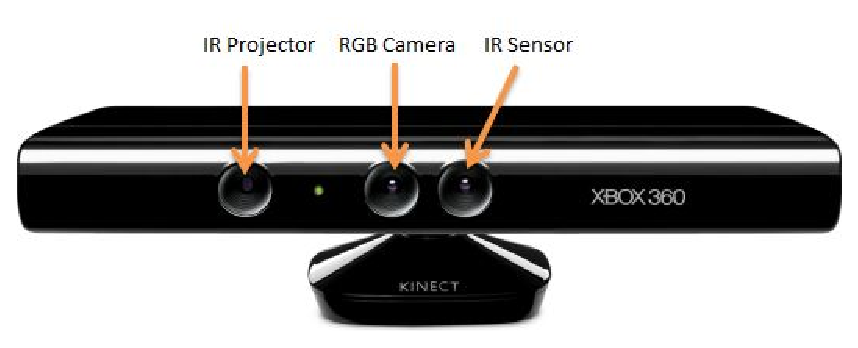
\includegraphics[scale=0.5]{img/kinect/kinect2.eps}
		% 	\caption[Kinect Sensors]{Kinect sensors: depth sensor and VGA camera location.}
		% 	\end{center}
		% \end{figure}


		The parts that compose the Kinect sensor are the following: 

		\begin{itemize}
			\item{\textbf{VGA camera}}\\
			The camera contained by the kinect has a pixel resolution of 640x480 and a frame rate of 30 fps. It is used mainly to provide the output data with the RGB components for each point. 
			
			\item{\textbf{Depth sensor}\\
			The depth sensor consists on an infra-red projector combined with a monochrome CMOS sensor. This latter measures the time it takes the light to come back after being reflected on the objects. Knowing the speed of light it can be easily obtained the distance of the objects from the depth sensor. 

			\item{\textbf{Multi-array microphone}}\\
			This array of four microphones are included because the kinect was designed as a gaming device. They are not used for the three-dimensional world retrieving. 

		\end{itemize}


\newpage
%%%%%%% SOFTWARE NODES %%%%%%
\addcontentsline{toc}{subsection}{Software nodes}
\subsection{Software nodes}

The processing needed to provide all the functionality is divided in nodes. Here they are presented, ordered using the data work-flow, beginning the ones using the raw input data to the system and finishing with the ones that deliver the output of the system. 
\\

\begin{itemize}
	\item{\textbf{\large Converter}}\\
This node is the first step of the code. It transforms the input data from the pi\_tracker package into the custom message used within the software. The information provided by that third-party code contains the position in the space of each joint of the body. The converter node takes only both hand's position. 
\\

It use case diagram of the node can be seen in the diagram below: 

\begin{figure}[h]
	\begin{center}
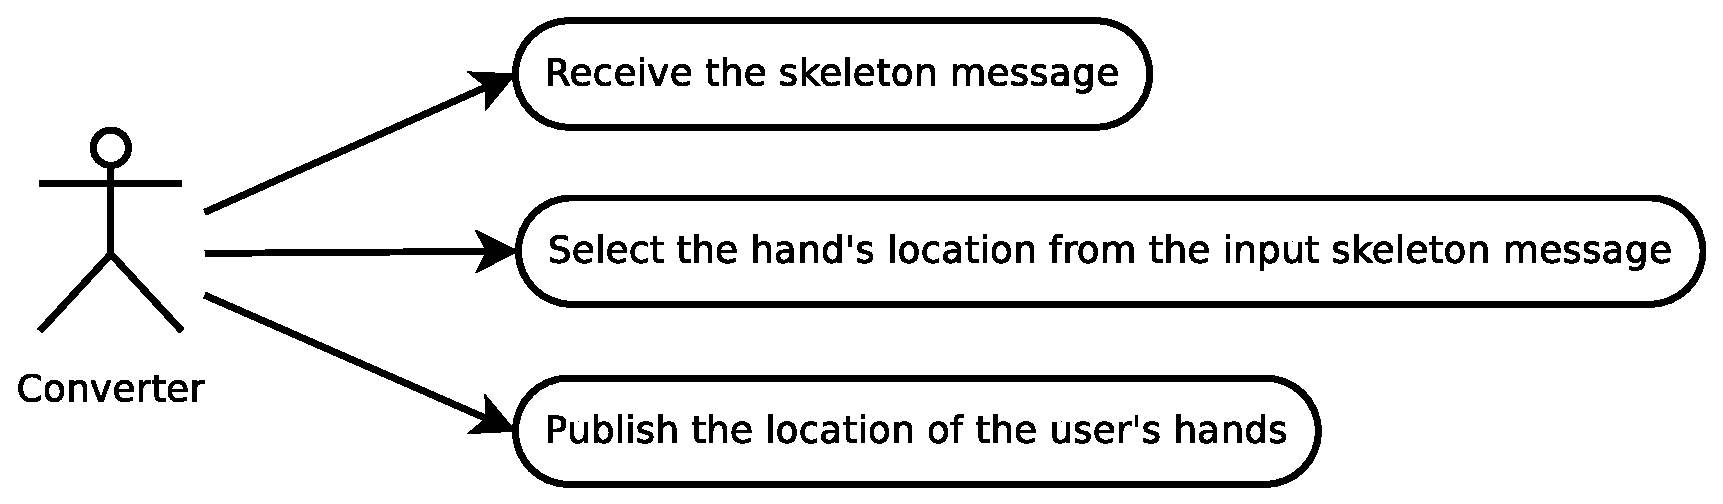
\includegraphics[scale=0.2]{img/diagrams/uc_converter.eps}
	\caption[Use case diagram converter node]{Use Case diagram of the converter node}
	\end{center}
\end{figure}

	
	\item{\textbf{ROI Segmenter 3D}}\\
The input of this node is the raw 3D information from the sensor and the hand's locations from the third-party package pi\_tracker, as well as the hand in which the user is holding the object. The node segments a prism from the original point cloud around the selected hand's center. The prism vertices coordinates are transformed from world coordinates to pixels. That information is the output of the node, together with the segmented point cloud. 

\begin{figure}[h]
	\begin{center}
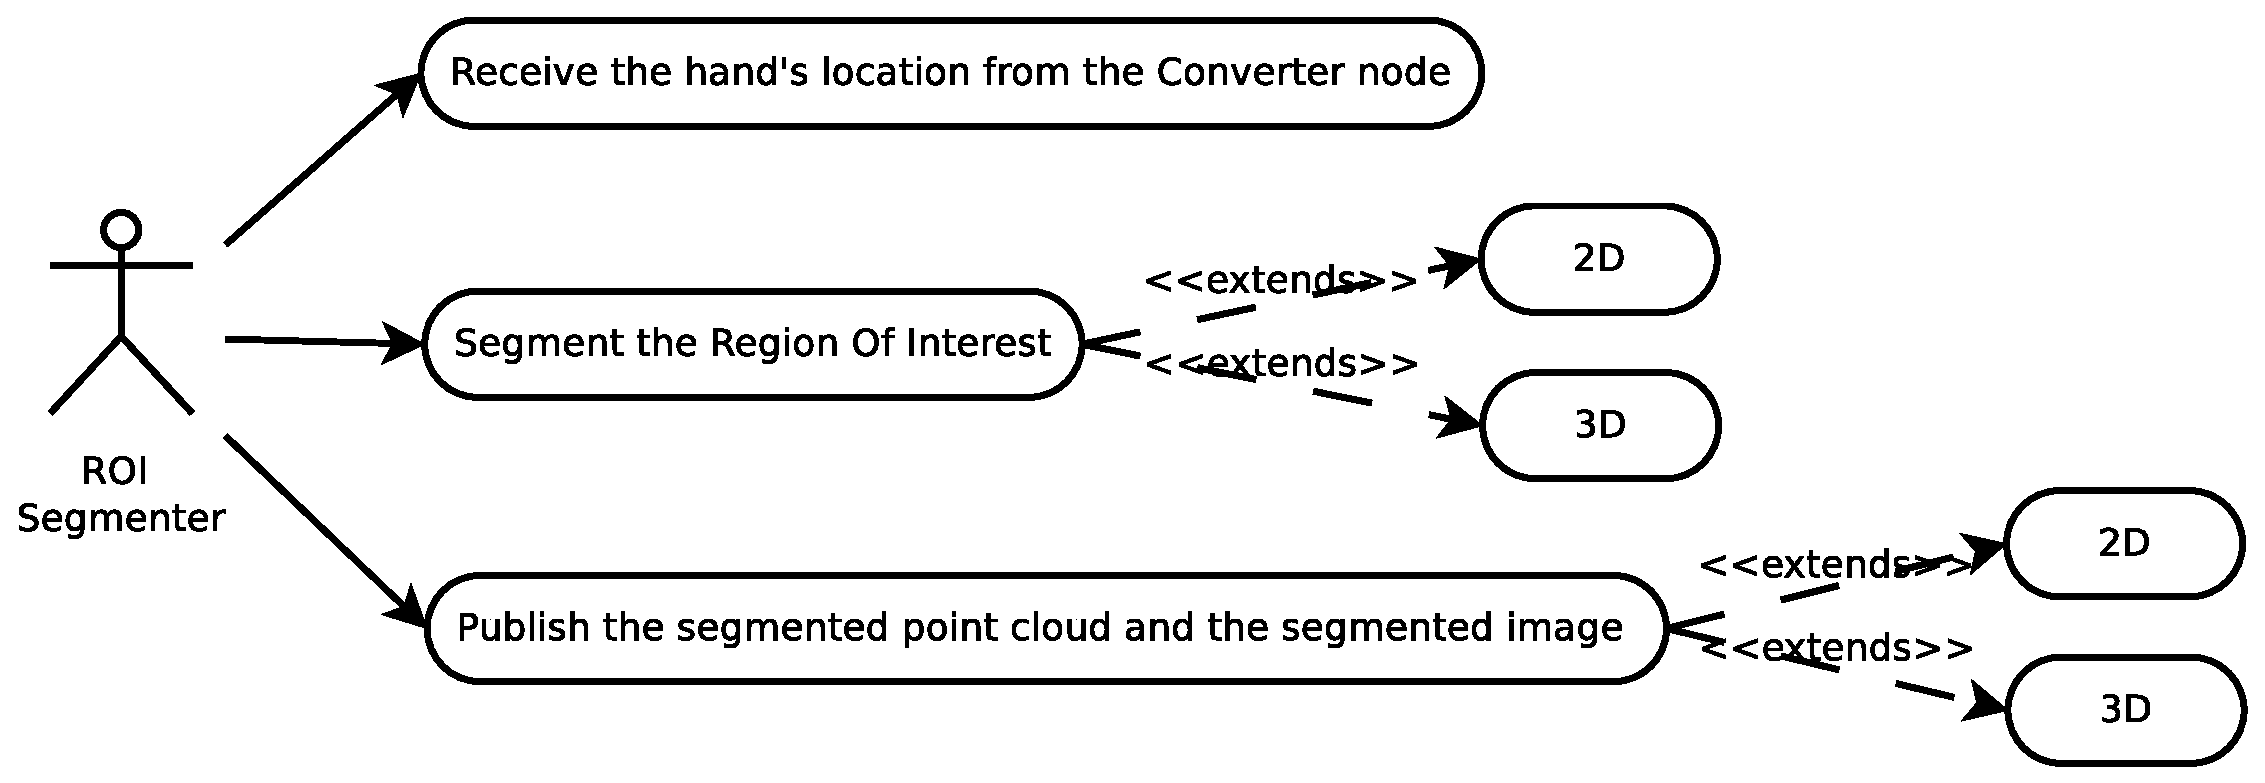
\includegraphics[scale=0.2]{img/diagrams/uc_roi_segmenter.eps}
	\caption[Use case diagram ROI segmenter 3D node]{Use Case diagram of the ROI segmenter 3D node}
	\end{center}
\end{figure}
 
	\item{\textbf{ROI Segmenter 2D}}\\
The present node takes as the input the raw 2D information from the RGB-D sensor and the hand's locations in pixels returned from the ROI segmenter 3D node. Then, it extracts the ROI (Region Of Interest) taking a square section around the center of the hand. The size of that figure is fixed for simplicity. Since due to the RGB-D sensor's current resolutions the user must remain at a fixed distance from the sensor, the difference in the scale due to the distance is negligible and hence the size can be fixed. 
\\

In the picture the use case diagram of the node can be observed.
\begin{figure}[h]
	\begin{center}
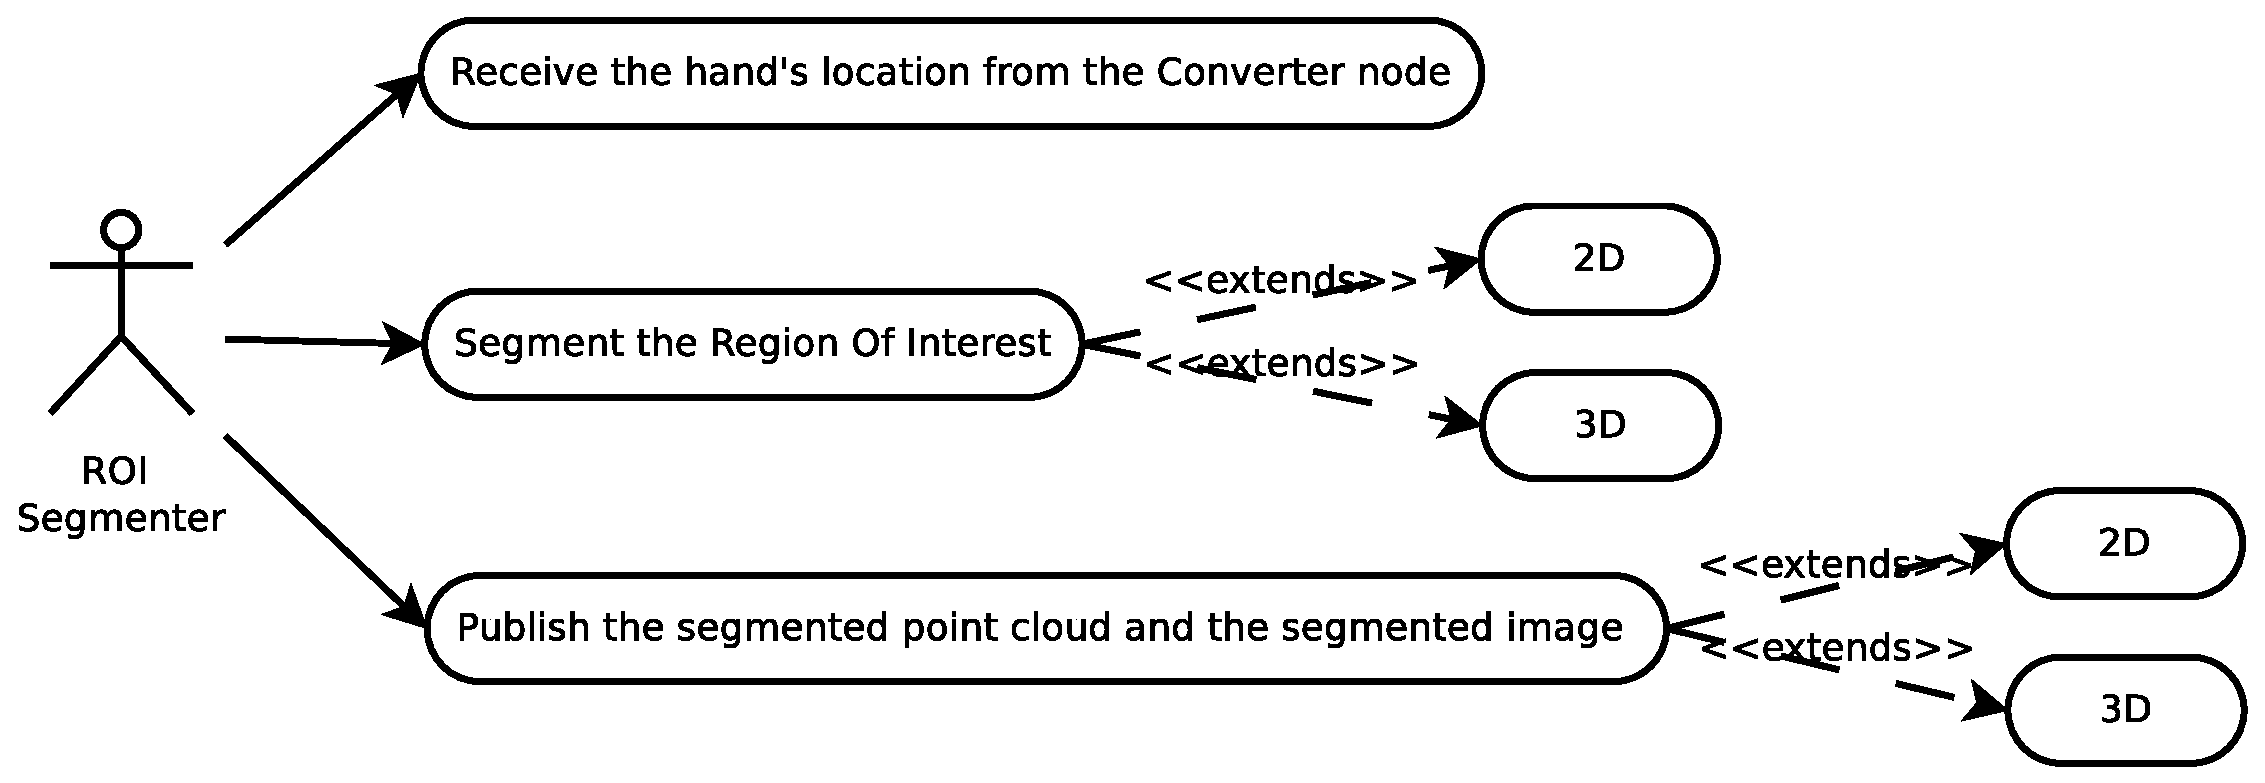
\includegraphics[scale=0.2]{img/diagrams/uc_roi_segmenter.eps}
	\caption[Use case diagram ROI segmenter 2D node]{Use Case diagram of the ROI segmenter 2D node}
	\end{center}
\end{figure}


	\item{\textbf{Feature Extractor 2D}}\\
This node takes as an input the segmented 2D ROI from the previous nodes and extracts the features. A feature is defined depending on the application and context of the computer vision project. In general, it is an interesting or important characteristic, point or region of an image. The application will determine which feature describes better the object of study. 
\\

The best feature or descriptor is that which has a higher repeatability, i.e the ability of obtaining the same output given different inputs. This is useful when making a feature matching to compare two object, which is the case in this project. 
\\

Hence, it can be seen that the recognition algorithm has as a bottle neck in its performance the repeatability of the features used to describe the different objects. 


	\item{\textbf{Feature Extractor 3D}}\\
	\item{\textbf{Event Handler}}\\
	\item{\textbf{Learner Recognizer}}\\
\end{itemize}

 




